% !TEX TS-program = pdflatex
% !TEX encoding = UTF-8 Unicode

% This is a simple template for a LaTeX document using the "article" class.
% See "book", "report", "letter" for other types of document.

\documentclass[20pt]{article} % use larger type; default would be 10pt

\usepackage[utf8]{inputenc} % set input encoding (not needed with XeLaTeX)

%%% Examples of Article customizations
% These packages are optional, depending whether you want the features they provide.
% See the LaTeX Companion or other references for full information.

%%% PAGE DIMENSIONS
\usepackage{geometry} % to change the page dimensions
\geometry{a4paper} % or letterpaper (US) or a5paper or....
% \geometry{margin=2in} % for example, change the margins to 2 inches all round
% \geometry{landscape} % set up the page for landscape
%   read geometry.pdf for detailed page layout information

\usepackage{graphicx} % support the \includegraphics command and options

% \usepackage[parfill]{parskip} % Activate to begin paragraphs with an empty line rather than an indent

\usepackage{amsmath} % apparently this helps with set notation
\usepackage{amssymb}

%%% PACKAGES
\usepackage{booktabs} % for much better looking tables
\usepackage{array} % for better arrays (eg matrices) in maths
\usepackage{paralist} % very flexible & customisable lists (eg. enumerate/itemize, etc.)
\usepackage{verbatim} % adds environment for commenting out blocks of text & for better verbatim
%\usepackage{subfig} % make it possible to include more than one captioned figure/table in a single float
\usepackage{mathtools}
\usepackage{graphicx} % supports images in latex
% These packages are all incorporated in the memoir class to one degree or another...

\usepackage{graphicx}
\usepackage{subcaption}

%%% Other stuff
\DeclarePairedDelimiter\ceil{\lceil}{\rceil}
\DeclarePairedDelimiter\floor{\lfloor}{\rfloor}

%%% HEADERS & FOOTERS
\usepackage{fancyhdr} % This should be set AFTER setting up the page geometry
\pagestyle{fancy} % options: empty , plain , fancy
\renewcommand{\headrulewidth}{0pt} % customise the layout...
\lhead{}\chead{}\rhead{}
\lfoot{}\cfoot{\thepage}\rfoot{}

%%% SECTION TITLE APPEARANCE
\usepackage{sectsty}
\allsectionsfont{\sffamily\mdseries\upshape} % (See the fntguide.pdf for font help)
% (This matches ConTeXt defaults)

%%% ToC (table of contents) APPEARANCE
\usepackage[nottoc,notlof,notlot]{tocbibind} % Put the bibliography in the ToC
\usepackage[titles,subfigure]{tocloft} % Alter the style of the Table of Contents
\renewcommand{\cftsecfont}{\rmfamily\mdseries\upshape}
\renewcommand{\cftsecpagefont}{\rmfamily\mdseries\upshape} % No bold!

%%% graphics path


%%% END Article customizations

%%% nice things to keep around
%\begin{figure}[!htbp]
%  	\centering
%   	\begin{subfigure}[p]{0.5\linewidth}
%    	\includegraphics[width=\linewidth]{}
%	\caption{figure 1}
%	\label{fig:sub1}
%   	\end{subfigure}
%\end{figure} 

% \noindent\rule{2cm}{0.4pt} 
%%% puts a small horizontal line

% \mathcal{O} 
%%% big O notation

%%% The "real" document content comes below...

\title{Research Topic Intro: Mandlebrot Set}
\author{Liam Dillingham}
%\date{} % Activate to display a given date or no date (if empty),
         % otherwise the current date is printed 

\begin{document}
\maketitle

\section{Background}

The Mandlebrot Set is a set of numbers that fulfill the constraints of an equation iterated on the complex plane.  We can define the Mandlebrot Set as: \\ 

$W = \{ c \in \mathbb{C} \mid \forall n \leq N, |z| \leq 2; \text{ where }  f_c^{n}(z) = z^{2}+c\}$. \\ 

That is, the Mandlebrot set is all complex numbers such that given the equation \\$f_c^{n}(z) = z^{2}+c$, the output of this equation, $z$, has a magnitude $\leq 2$ for every iteration up to and including $N$.  Note that the "exponent" on $f_c^{n}$ does not mean we take the power of it, but rather it is the number of iterations of the function on $c$, feeding the output $z$ from the $i$th iteration into the $i+1$ iteration, and where $c$ is the selected complex number we wish to test on. \\ 

The Mandlebrot Set's interest comes from the visualization of it, where points in the complex plane that are accepted are colored black, and points rejected by the set's constraints are colored white.  Note that since this is usually calculated on a computer, we always have some margin of error where we are accepting points into the set that violate the constraints of the set, since it may take an arbitrarily large number of iterations to grow past the bounding.  Note also that we don't bother computing any points $<-2$ or $>2$ since their magnitude violates the condition initially.  

\begin{figure}[!htbp]
  	\centering
   	\begin{subfigure}[p]{0.5\linewidth}
    	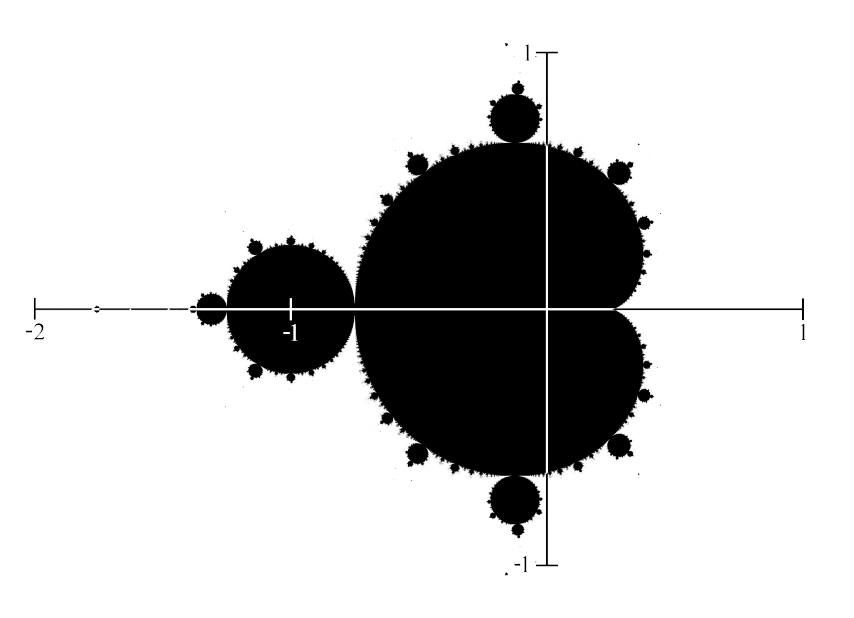
\includegraphics[width=\linewidth]{./figures/Mandelset_simple.png}
	\caption{Simple drawing of Mandlebrot Set coloring}
	\label{fig:sub1}
   	\end{subfigure}
\end{figure} 

The set becomes more interesting as we observe the boundary, where the slightest adjustment $\epsilon$ in the values can produce wildly different results in the acceptance of a point. In addition, by increasing the number of iterations to an arbitrarily large degree, we improve the accuracy of acceptance and improve the level of detail of the boundary.  We can improve our understanding of the growth of the values under the equation $f_c^{n}$ by adding color to the visualization. \\ 

We color points that grow larger than 2 quickly red, and points that grow slowly violet, while all other colors are given to the different intermediate rates.  The number of iterations that qualifies a point as being red depends on the proportion it takes from our limit, $N$.  Remember than any point that does not exceed 2 at $N$ iterations is painted black and in the set.

\end{document}










































